\documentclass[10pt,a4paper]{amsart}
\usepackage[margin=19mm]{geometry}
\usepackage{amsmath,amssymb,mathtools}
\usepackage[scr=rsfs,cal=euler]{mathalfa}
\usepackage{xfrac}
\usepackage[unicode,hidelinks,bookmarks=false]{hyperref}
\newcommand{\ie}{i.e.\ }
\newcommand{\cf}{cf.\ }
\newcommand{\resp}{respectively\ }
\newcommand{\Subsection}{\subsection}
\providecommand{\nobreakdash}{\nobreak\hbox{-}}
\setlength{\emergencystretch}{2em}
\multlinegap0pt
\usepackage{tikz}
\usetikzlibrary{cd}
\usepackage{tikz}
\usepackage{mathtools}
\usepackage{float}
\usepackage{amssymb}
\usepackage[shortlabels]{enumitem}
\usepackage{xcolor}
\newtheorem{theorem}{Theorem}
\usepackage{cleveref}
\crefname{theorem}{Theorem}{Theorems}
\newcommand{\im}{\textup{im}} 
\title{Homological methods in rigidity theory using graphs of groups}
\author{Joannes Vermant}
\date{Source: arXiv:2603.05435v2 (CC BY 4.0)}
\begin{document}
\maketitle

\noindent\emph{Source and licence.} Homological methods in rigidity theory using graphs of groups. Version arXiv:2603.05435v2 (CC BY 4.0), distributed by arXiv under the Creative Commons Attribution 4.0 International licence, http://creativecommons.org/licenses/by/4.0/, as recorded in the arXiv licence metadata for this exact version and shown on the abstract page https://arxiv.org/abs/2603.05435v2. Full licence notice: \texttt{licenses/arxiv-2603.05435-CC-BY-4.0.txt}.\par\smallskip

\noindent\textit{Editorial scope.} Counted unit: the article's theorem Extension-for-sheaves (source0.tex lines 662--677). The article's complete original proof of it is delivered with it (source0.tex lines 678--830, one \texttt{proof} environment of 153 lines). No mathematics is written, repaired or re-derived: the statement and the proof are the article's own lines, in the article's own notation, and no retained line is substituted or re-flowed.  Retained uncounted as the source-local context the proof needs: lines 547--549; lines 618--620.  Nothing was omitted from any retained span, so the package carries no omission record.  No retained line contains a citation, so the wrapper carries no bibliography and no bibliography entry.  The retained lines contain the article's own diagram code, which the wrapper typesets with the standard tikz packages; no image file is delivered and the package declares no asset dependency.  Editorial formatting only, in addition: an AMS \texttt{amsart} preamble that restates the article's own declarations and macros used by the retained lines, namely the environments \texttt{theorem} on separate counters, together with the standard packages those lines need.  The retained environments print in this document as Theorem 1 in order of appearance, whereas the article prints the same items with the numbering of its own full document.  The complete native source of the article as distributed in the arXiv e-print for this exact version is bundled unchanged as \texttt{sources/195802/source0.tex}.
\begin{equation}\label{eq: les-ass}
    0 \rightarrow \mathcal{S} \rightarrow \underline{\mathbb{V}} \rightarrow \mathcal{F} \rightarrow 0. 
\end{equation}

\begin{equation} \label{eq: rule for h1}
    \sum_{e\in E} w_e = \sum_{e\in E} w_e + \sum_{e: v_0\in e} [v_0: e] w_{v_0}.
\end{equation}

\begin{theorem}\label{Extension-for-sheaves}
    Suppose that $s < n/2$, and let $d = n-s$.
    Let $\Gamma =(V, E)$ be a multi-graph, and suppose $\mathcal{F} = \underline{\mathbb{V}}/\mathcal{S} \in Z_{s, n}(\Gamma)$ such that $h^{1}(\mathcal{F}) = 0$. Suppose that $\Gamma'$ results from applying a $d$-dimensional $k$-extension, with new vertex $v_{*}$, new edges $f_{1} =u_{1}v_{*}, f_{2}=u_{1}'v_{*},\dots, f_{2k +1}=v_{1}v_*, \dots, f_{d+k}=v_{d-k}v_*$,  and deleted edges $e_1=u_1u_1',\dots, e_k=u_ku_k'$. If $\mathcal{F}' = \underline{\mathbb{V}}/ \mathcal{S}'$, is constructed using $\mathcal{S}'$ where 
    \begin{align*}
        \mathcal{S}'(x) &= \mathcal{S}(x) \textup{ if }  x\in V,
    \end{align*}
    and
    \begin{equation*}
    \begin{array}{clr}
        \mathcal{S}'(f_{2j -1}) &= \ker(\alpha_{e_j})  &\textup{for $j \in\{1, \dots, k\}$}\\
        \mathcal{S}'(f_{2j}) &= \ker(\alpha_{e_j})  &\textup{for $j \in\{1, \dots, k\}$}\\
        \mathcal{S}'(f_{j}) &= \ker(\alpha_{j}) &\textup{for some $\alpha_{j} \in \mathbb{V}^{*}$ whenever $j \in\{2k+1, \dots, k + d\}$}
        \end{array}
    \end{equation*}
    such that $\alpha_{e_1}, \dots, \alpha_{e_k}, \alpha_{k+1},\dots,\alpha_{d}$ are linearly independent, and if $$\mathcal{S}'(v_*) = \bigcap_{i=1}^{k}  \ker(\alpha_{e_i}) \cap  \bigcap_{j=k+1}^{d}  \ker(\alpha_{j}),$$ then one has $h^{1}(\mathcal{F}') = 0$ and $\mathcal{F}'\in Z_{s, n}(\Gamma')$. 
\end{theorem}

\begin{proof}
 We will use the notation $\alpha_{i} = \alpha_{e_i}$ whenever $i\leq k$. Let us first note that defining $\mathcal{S}'(v_*) = \bigcap_{j=1}^{d}  \ker(\alpha_{j})$ yields a sheaf $\mathcal{F}' \in Z_{s, n}(\Gamma')$ since $\dim( \bigcap_{j=1}^{d} \ker(\alpha_{j})) = n - d = s$. We orient all edges towards the vertex $v_*$, and orient all edges $u_i'u_i$ from $u_i'$ towards $u_i$.

One has the long exact sequence from the short exact sequence \eqref{eq: les-ass}
\begin{equation*}
    \begin{array}{cl}
    0 \rightarrow & H^0(\Gamma', \mathcal{S}') \rightarrow H^0(\Gamma', \underline{\mathbb{V}}) \rightarrow H^0(\Gamma', \mathcal{F}') \\[10pt]
    &\xrightarrow{\delta} H^1(\Gamma', \mathcal{S}') \rightarrow H^1(\Gamma', \underline{\mathbb{V}}) \rightarrow H^1(\Gamma', \mathcal{F}') \rightarrow 0.
\end{array}
\end{equation*}
Thus, $H^{1}(\Gamma', \mathcal{F}') = 0$ if and only if $H^1(\Gamma', \mathcal{S}') \rightarrow H^1(\Gamma', \underline{\mathbb{V}})$ is surjective, and one has the same for the graph $\Gamma$. We will show that this map is surjective. We thus seek to find $ (w_{e})_{e \in E} \in H^1(\Gamma', \mathcal{S}')$ that map onto an arbitrarily given element of $H^{1}( \Gamma', \underline{\mathbb{V}})$. Up to $\im(d)$, elements of $H^{1}( \Gamma', \mathcal{S}')$ are given by formal sums $\sum_{e\in E(\Gamma')} s_e$, where $s_e\in \mathcal{S}'(e)$.
We will first treat two special cases, which we will then use together with the surjectivity of $H^{1}(\Gamma, \mathcal{S}) \rightarrow H^{1}(\Gamma, \underline{\mathbb{V}})$, to show that $H^{1}(\Gamma', \mathcal{S}') \rightarrow H^{1}(\Gamma', \underline{\mathbb{V}})$ is surjective.\\
We consider first cochains that are nonzero only on an added edge $f_{j}$ with $j > 2k$, and equal to $W$ on this edge. We denote the cochain by $W_{f_{j}}$. Since the elements $\alpha_{1}, \dots, \alpha_{k}, \alpha_{k+1} , \dots, \alpha_{d}$ are linearly independent, we have $\bigcap_{c \neq j-k} \ker(\alpha_c) + \ker(\alpha_{j-k}) = \mathbb{V}$, where $\alpha_{j-k}$ corresponds to the edge $f_j$. Thus there exist elements $w_{*} \in \bigcap_{c \neq j-k} \ker(\alpha_c)$ and a $w_{j-k} \in \ker(\alpha_{j-k})$ such that 
\begin{equation*}
    w_{*}  + w_{j-k} = W_{f_j}. 
\end{equation*}
  Now, consider the cochain defined by (see also \Cref{fig: proof_case_1}):
\begin{equation*}
\begin{array}{clcc}
    w_{f_{c}} &= - w_{*}  & \textup{if } c \in \{1, \dots, d+k\} \setminus \{j\} \\
    w_{f_{j}} &= w_{j-k}  & \\
    w_{e} &=0  &\textup{ otherwise.}
\end{array}
\end{equation*}
It is clear that this cochain defines an element of $H^{1}( \Gamma', \mathcal{S}')$. Moreover, one can see by using equation \eqref{eq: rule for h1} at $v_*$ with $w_{*}$, that it is equivalent to $W_{f_j}$, which is precisely what we needed to show.
\begin{figure}[h!]
\centering
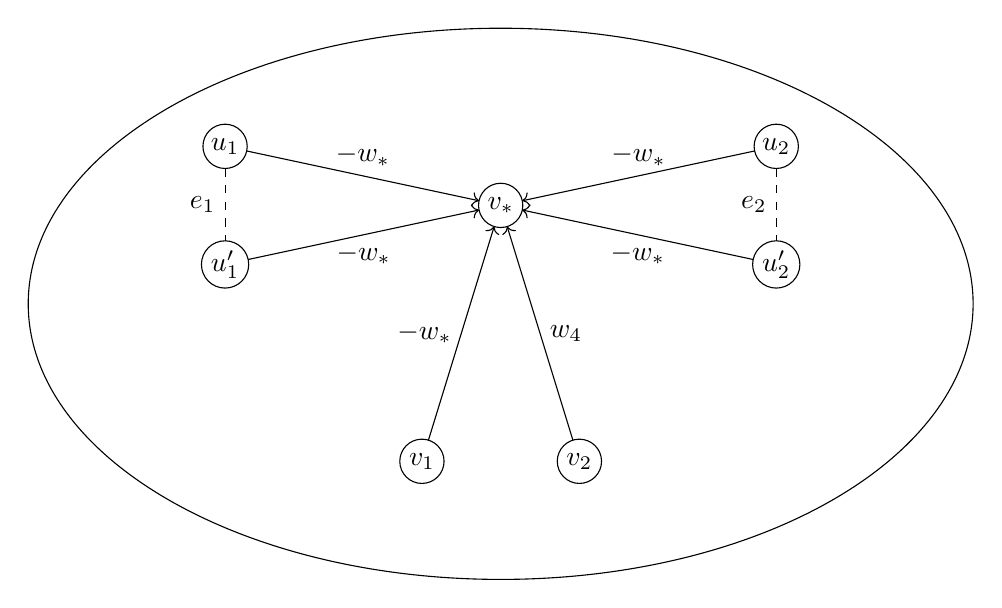
\begin{tikzpicture}
\tikzstyle{vertex}=[circle, draw, fill=white, minimum size=16pt, inner sep=1pt, outer sep=0pt]
\tikzstyle{dot}=[fill=black, circle, inner sep=1.5pt]
\draw (0,0) ellipse (6cm and 3.5cm);
\node[vertex] (vstar) at (0,1.25)  {$v_*$};
\node[vertex] (v1) at (-3.5,2)  {$u_1$};
\node[vertex] (v2) at (-3.5,.5)  {$u_1'$};
\node[vertex] (v3) at (3.5,2)  {$u_2$};
\node[vertex] (v4) at (3.5,.5)  {$u_2'$};
\node[vertex] (v5) at (-1, -2)  {$v_1$};
\node[vertex] (v6) at (1, -2)  {$v_2$};


\draw[dashed]  (v1) -- (v2)  node[midway, left, draw=none, fill=none] {$e_1$};
\draw[dashed]  (v3) -- (v4)  node[midway, left, draw=none, fill=none] {$e_2$};
\draw[->] (v1) -- (vstar) node[midway, above, draw=none, fill=none] {$-w_*$};
\draw[->] (v2) -- (vstar) node[midway, below, draw=none, fill=none] {$-w_*$};
\draw[->] (v3) -- (vstar) node[midway, above, draw=none, fill=none] {$-w_*$};
\draw[->] (v4) -- (vstar) node[midway, below, draw=none, fill=none] {$-w_*$};
\draw[->] (v5) -- (vstar) node[midway, left, draw=none, fill=none] {$-w_*$};
\draw[->] (v6) -- (vstar) node[midway, right, draw=none, fill=none] {$w_4$};
\end{tikzpicture}
\caption{An illustration of the cochain for the first case for the $4$-dimensional $2$-extension. Edges not involved in the $2$-extension are not pictured. The edges $e_1$ and $e_2$ are replaced, and edges $f_1,\dots, f_6$ are added. The picture illustrates the construction of the cochain equal to $W_{f_{6}}$, where $f_6$ is the edge between $v_2$ and $v_*$.}
\label{fig: proof_case_1}
\end{figure}

We now consider elements of the form $W_{f_{2j -1}} + W_{f_{2j}}$ with $j\leq k$, where $f_{2j-1},f_{2j}$ are given by $f_{2j-1} = v_*u_j, f_{2j} = v_*u_j'$, and they replace the edge $e_{j}$. By the linear independence assumption, we have $\bigcap_{c \neq j} \ker(\alpha_c) + \ker(\alpha_j) = \mathbb{V}$, and thus there exist elements $w_{*} \in \bigcap_{c \neq j} \ker(\alpha_c)$ and a $w_j \in \ker(\alpha_j)$ such that $w_* + w_j  = W$. One can then define a cochain
\begin{equation*}
\begin{array}{clcc}
    w_{f_{i}} &= - w_{*}  & \textup{if } i\in \{1, \dots, d+k\} \setminus \{2j, 2j-1\}\\
    w_{f_{2j-1}} &= w_{j}  & \\
    w_{f_{2j}} &= w_{j}  & \\
    w_{e} &=0  &\textup{ otherwise.}
\end{array}
\end{equation*}
 Again this cochain belongs to $H^{1}(\Gamma', \mathcal{S}')$, and using Equation \eqref{eq: rule for h1}, one can show that it maps onto $W_{f_{2j-1}} + W_{f_{2j}}$. See also the illustration in \Cref{fig: proof_case_2}.\\


\begin{figure}[h!]
\centering
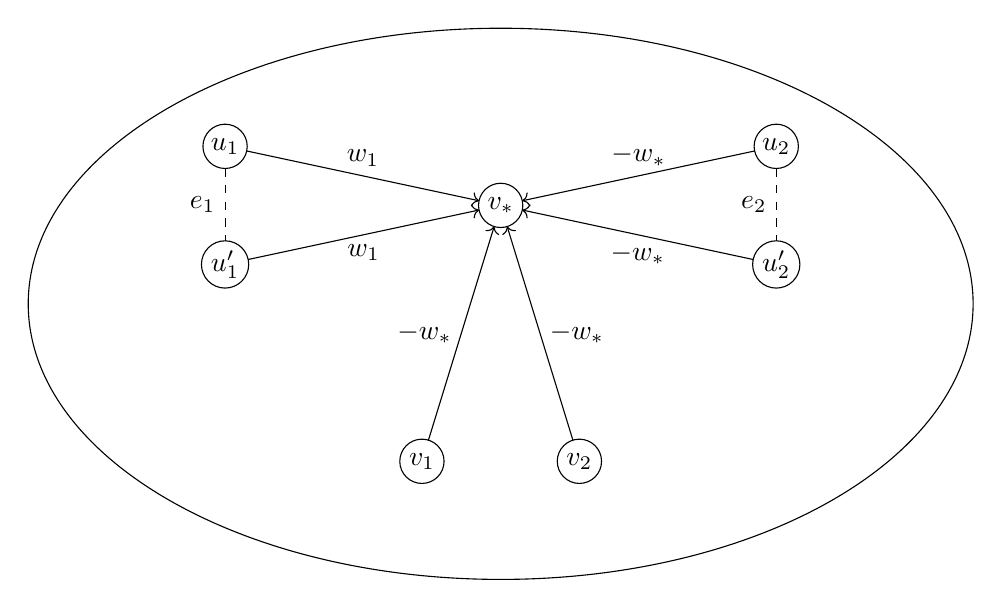
\begin{tikzpicture}
\tikzstyle{vertex}=[circle, draw, fill=white, minimum size=16pt, inner sep=1pt, outer sep=0pt]
\tikzstyle{dot}=[fill=black, circle, inner sep=1.5pt]
\draw (0,0) ellipse (6cm and 3.5cm);
\node[vertex] (vstar) at (0,1.25)  {$v_*$};
\node[vertex] (v1) at (-3.5,2)  {$u_1$};
\node[vertex] (v2) at (-3.5,.5)  {$u_1'$};
\node[vertex] (v3) at (3.5,2)  {$u_2$};
\node[vertex] (v4) at (3.5,.5)  {$u_2'$};
\node[vertex] (v5) at (-1, -2)  {$v_1$};
\node[vertex] (v6) at (1, -2)  {$v_2$};


\draw[dashed]  (v1) -- (v2)  node[midway, left, draw=none, fill=none] {$e_1$};
\draw[dashed]  (v3) -- (v4)  node[midway, left, draw=none, fill=none] {$e_2$};
\draw[->] (v1) -- (vstar) node[midway, above, draw=none, fill=none] {$w_1$};
\draw[->] (v2) -- (vstar) node[midway, below, draw=none, fill=none] {$w_1$};
\draw[->] (v3) -- (vstar) node[midway, above, draw=none, fill=none] {$-w_*$};
\draw[->] (v4) -- (vstar) node[midway, below, draw=none, fill=none] {$-w_*$};
\draw[->] (v5) -- (vstar) node[midway, left, draw=none, fill=none] {$-w_*$};
\draw[->] (v6) -- (vstar) node[midway, right, draw=none, fill=none] {$-w_*$};
\end{tikzpicture}
\caption{An illustration of the cochain for the second case for the $4$-dimensional $2$-extension. The picture illustrates the construction of the cochain equal to $W_{f_1} + W_{f_2}$.}
\label{fig: proof_case_2}
\end{figure}
To complete the proof, we will use the independence of $\mathcal{F}$ on $\Gamma$ and the two cases that we have considered to show that the map is surjective in general. Let $N$ be the vector subspace of $H^{1}(\Gamma', \underline{\mathbb{V}})$ generated by 
\begin{equation*}
    W_{f_{i}}, W_{f_{2j-1}} + W_{f_{2j}},
\end{equation*}
  where $W\in \mathbb{V}$ and $j\in \{1, \dots, k\}$ and $i \in \{2k+1, \dots k + d\}$. From the above two cases, we know that
  \begin{equation*}
  N \subseteq \im(H^{1}(\Gamma', \mathcal{S}') \rightarrow H^{1}(\Gamma', \underline{\mathbb{V}})).
  \end{equation*}

Define a linear map
\begin{equation*}
\begin{array}{cl}
   \varphi: & \oplus_{e \in E(\Gamma)}  \mathcal{S}(e) \rightarrow \oplus_{e \in E(\Gamma')} \mathcal{S}'(e):\\
   
   &\begin{cases}
    W_{e} \mapsto W_{e} &\text{ if $e\in E(\Gamma) \cap E(\Gamma') $}\\
   W_{e_i} \mapsto W_{f_{2i - 1}} &\text{ if $e_i=u_iu_{i}'$ is a deleted edge},\\
   \end{cases}
\end{array}
\end{equation*}
and by extending linearly to all other vectors. This is clearly well defined. We define another linear map
\begin{equation*}
\begin{array}{cl}
   \psi: &H^{1}(\Gamma, \underline{\mathbb{V}}) \rightarrow H^{1}(\Gamma', \underline{\mathbb{V}})/N:\\
   &\begin{cases}
    W_{e} \mapsto W_{e} &\text{ if $e \in E(\Gamma) \cap E(\Gamma')$}\\
    W_{e} \mapsto W_{f_{2i -1}} &\text{ if $e_i=u_iu_{i}'$ is a deleted edge,}
    \end{cases}
\end{array}
\end{equation*}
and by extending linearly to all other vectors.
We need to check that $\psi$ is well-defined. By \eqref{eq: rule for h1}, it suffices to check that for each vertex $v$, if $\sum_{e\in N(v)} A_{e} = \sum_{e\in N^{+}(v)} (A_{e} + H)+ \sum_{e\in N^{-}(v)} (A_{e} - H)$ in $H^{1}(\Gamma, \underline{\mathbb{V}})$, then
\begin{equation*}
    \psi \left(\sum_{e\in N(v)} A_{e}\right) = \psi\left( \sum_{e\in N^{+}(v)} (A_{e} + H)+ \sum_{e\in N^{-}(v)} (A_{e} - H)\right)
\end{equation*}
in $H^{1}(\Gamma', \underline{\mathbb{V}})/N$. 
Thus, let $v$ be a vertex and suppose that $v$ is the terminal vertex of $e_{i_1}, \dots e_{i_{a}}$ and the initial vertex of $e_{i_{a+1}}, \dots e_{i_{b}}$ for some deleted edges $e_{i_1}, \dots e_{i_b}$, and that additionally, the edges $f_{j_1}, \dots, f_{j_c}$ are adjacent to $v$ (with $j_i \geq 2k$ for $i\in \{1, \dots, c\}$). Denote $S= \{e_{i_1}, \dots e_{i_{b}}, f_{j_1},\dots, f_{j_c} \}$. 
We have
\begin{align*}
\psi(\left(\sum_{e\in N_{\Gamma'}(v)} A_{e}\right) ) &= \sum_{p = 1}^{a} A_{f_{2  i_{p} - 1}} + \sum_{p = a+1}^{b} A_{f_{2  i_{p} - 1}} + \sum_{e\in N_{\Gamma'}^{+}(v) \setminus S}  A_{e} + \sum_{e\in N_{\Gamma'}^{-}(v) \setminus S}  A_{e} \\
&= \sum_{p = 1}^{a} (A_{f_{2  i_{p} - 1}} - H) - \sum_{p = a+1}^{b} (A_{f_{2  i_{p}}} +H) + \sum_{f_{j_q}}( - H)\\
&+ \sum_{e\in N_{\Gamma'}^{+}(v) \setminus S}  (A_{e} + H)+ \sum_{e\in N_{\Gamma'}^{-}(v) \setminus S}  (A_{e} -H)\\
&= \sum_{p = 1}^{a} (A_{f_{2  i_{p} - 1}} - H) + \sum_{p = a+1}^{b} (A_{f_{2  i_{p} -1}} + H) + \psi(\sum_{e\in N_{\Gamma'}(v) \setminus S}  (A_{e} \pm H)) \\
&=  \psi\left( \left(\sum_{e\in N_{\Gamma'}^{+}(v)} A_{e} + H\right) + \left(\sum_{e\in N_{\Gamma'}^{-}(v)} A_{e} - H\right)\right)
\end{align*}

We have used the first case above for the terms $H$ supported on $f_{j_{q}}$, since these belong to $N.$ We used $W_{f_{2j}} = -W_{f_{2j -1}} \textup{mod } N$, which follows from the second case, in the second and third equality. The map is thus well-defined. The map $\psi$ is surjective since, for any edge $e$, either $W_{e}$ obviously lies in the image, or $W_{e} \in N$, or $e=f_{2i}$ with $i\leq k$, in which case $W_{f_{2i}} = -W_{f_{2i -1}}$ clearly lies in the image.

Now note that the following diagram commutes:
\begin{figure}[h!]
    \centering
\begin{tikzcd}
\oplus_{e\in E(\Gamma)} \mathcal{S}(e) \arrow[r, "\varphi"] \arrow[d, "\textup{ mod } d"] & \oplus_{e \in E(\Gamma')} \mathcal{S}'(e) \arrow[d, " \textup{ mod } d"]  \\
H^{1}(\Gamma, \mathcal{S})  \arrow[d] & H^{1}(\Gamma', \mathcal{S}') \arrow[d] 
\\
{H^{1}(\Gamma, \underline{\mathbb{V}})} \arrow[r, "\psi"] & {H^{1}(\Gamma', \underline{\mathbb{V}})/N}
\end{tikzcd}
\end{figure}

The map $H^{1}(\Gamma, \mathcal{S})\rightarrow H^{1}(\Gamma, \underline{\mathbb{V}})$ is surjective by our assumption since $H^{1}(\Gamma, \mathcal{F}) = 0$ and by the long exact sequence associated to \eqref{eq: les-ass}. Thus, the composite map $\oplus_{e \in E} \mathcal{S}(e) \rightarrow H^{1}(\Gamma', \underline{\mathbb{V}})/N$ (going the bottom-left path in the diagram) is surjective as well since all maps involved are surjective. Thus, the map $H^{1}(\Gamma', \mathcal{S}') \rightarrow  H^{1}(\Gamma', \underline{\mathbb{V}})/ N$ must be surjective as well. By the two special cases, we see that $N$ is in the image of the map $H^{1}(\Gamma, \mathcal{S}) \rightarrow H^{1}(\Gamma', \underline{\mathbb{V}})$. Then, we see that the map $H^{1}(\Gamma', \mathcal{S}') \rightarrow H^{1}(\Gamma', \underline{\mathbb{V}})$ is surjective, completing the proof of the theorem.
\end{proof}

\end{document}
